\documentclass[./main.tex]{subfiles}
\graphicspath{{\subfix{./Abbildungen/}}}
\begin{document}
\renewcommand{\tasktitle}{Komische Chemie}
\renewcommand{\taskpoints}{76}
\renewcommand{\taskweight}{2} 
\aufgabenanfang

\blindtext
\FPprint\teilaufgabenpunkte
\teilaufgabe{\op{Zeichne} das Diagramm.}{}

\kasten{8cm}{
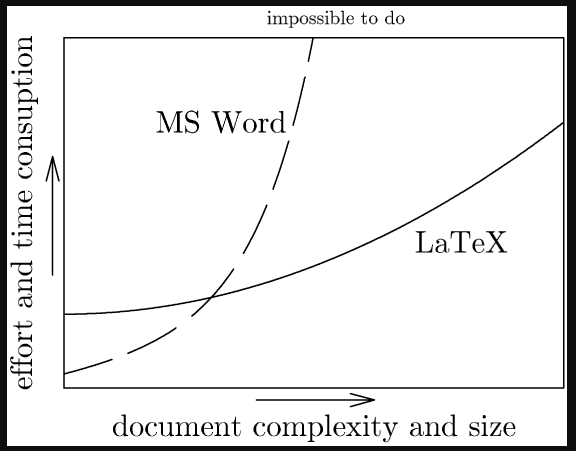
\includegraphics[width=0.5\linewidth]{test.png} \\ 
Achsen\punkte{2.5}, Graphen\punkte{1.5}, Wenn keine Pfeile -1 P.
}


Wenn man eine quadratische Gleichung aufstellt, dann sieht sie so aus wie in \eqref{A:Abb-BSP2} aus:

\begin{align}
    y = m\cdot x^2 + a \label{A:Abb-BSP2}
\end{align}

\teilaufgabe{\op{Trinke} 5 Bier.}{}

\kasten{5cm}{
    1. Bier \punkte{4.4}
    2. Bier \punkte{9.4}
    3. Bier \punkte{14.4}
    4. Bier \punkte{19.4}
    5. Bier \punkte{24.4}
}{}
\teilaufgabe{\op{Kreuze} die durch 4 teilbaren Antwort(en) \op{an}.\punkte{1}}{Es ist Antwort 4.}
\letzteantwort{}\MC{Antwort 1}{}{Antwort 2}{}{Antwort 3}{}{Antwort 4}{1}{Antwort 5}
Hier geht die Aufgabe weiter. 
\begin{scheme}[H]
 \centering
 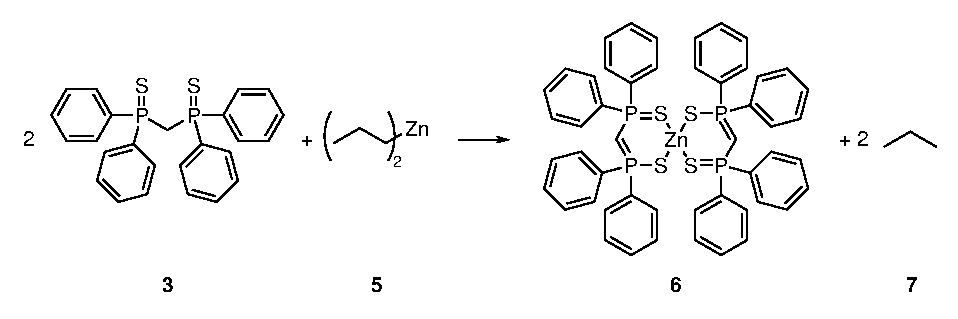
\includegraphics{Komplex.eps}
 \caption{Nochmal die Synthese.}
\end{scheme}

\aufgabenende
\end{document}
